\documentclass{beamer}
%
% Choose how your presentation looks.
%
% For more themes, color themes and font themes, see:
% http://deic.uab.es/~iblanes/beamer_gallery/index_by_theme.html
%
\mode<presentation>{
  \usetheme{Marburg}      % or try Darmstadt, Madrid, Warsaw, ...
  \usecolortheme{default} % or try albatross, beaver, crane, ...
  \usefonttheme{default}  % or try serif, structurebold, ...
  \setbeamertemplate{navigation symbols}{}
  \setbeamertemplate{caption}[numbered]
}

\usepackage[english]{babel}
\usepackage[utf8]{inputenc}
\usepackage[T1]{fontenc}

% Manually added
\usepackage{natbib}

\title{Automatic Summarization of Long Documents}
\author[Naman Chhibbar]{
  Naman Chhibbar \\
  \scriptsize advised by Dr. Jugal Kalita
}
\institute{
  Indian Institute of Technology, Hyderabad \\
  University of Colorado, Colorado Springs
}
\date{\today}

\begin{document}

\begin{frame}
  \titlepage
\end{frame}

\section{Introduction}
\label{sec:introduction}

Due to the ever-increasing amount of textual data available online, document summarization has become crucial for the efficient and accurate extraction of relevant information.
Large Language Models (LLMs) based on the transformer architecture \cite{vaswani2017attention} have shown outstanding abilities in many NLP tasks, including document summarization \cite{yadav2023state}.
Recent developments have demonstrated remarkable improvements in the relevancy and coherence of summaries generated by such LLMs.

However, long document summarization, which involves removing redundancies and makes reading long texts concise and efficient, remains a major challenge.
One of the significant limitations in the transformer architecture is limited context size, stemming from the quadratic memory and computational complexity of the attention mechanism \cite{du2023improving}.
This constraint hinders extracting relevant information from extensive texts where summarization is valuable to overcome the time, effort, and interpretive issues posed by complex and large documents.

We experiment with three novel approaches to address the input size limitations of transformers.
The methods introduced do not include any architectural modifications to the model used and can be incorporated into any existing pipeline.
We believe that these methods can effectively utilize the full potential of any existing LLM by capturing information from crucial aspects of the document.
Though our experiments only include the task of summarization, we hypothesize that our methods can be applied to NLP tasks that require processing long texts.

We start by stating the problem statement (\autoref{sec:problem}) and discussing related works (\autoref{sec:related-works}) to gain insights into the problem and the state-of-the-art solutions.
We then introduce the datasets (\autoref{sec:datasets}) and methodology (\autoref{sec:methodology}) used in our experiments.
For evaluating our results, we present some standard metrics (\autoref{sec:metrics}) used in text summarization.
We end the report by discussing our experimental findings (\autoref{sec:findings}) and potential future work (\autoref{sec:future-work}) and concluding the study (\autoref{sec:conclusion}).

\section{Problem Statement}


\begin{frame}{The Problem}

\begin{itemize}
	\item LLMs suffer from one major limitation: limited context size.
	\item<2-> This is due to the quadratic self-attention mechanism in the transformer
	architecture.
	\item<3-> For example, BERT has a context size of just 512 tokens (about half page
	of text).
	\item<4> Due to this, LLMs can not process long texts wherein summarization is
	valuable for efficient extraction of information.
\end{itemize}

\end{frame}

\section{Datasets}


\subsection*{GovReport}

Introduced by \citet{huang-etal-2021-efficient}, this dataset consists of
reports written by government research agencies, including the Congressional
Research Service and the U.S. Government Accountability Office.
Texts and summaries have an average word count of 7,700.71 and 451.36,
respectively, with a max word count of 73,815 and 1,442.
Figure \ref{fig:govreport} shows the word count distribution of the dataset.

\begin{figure}[!ht]
	\centering
	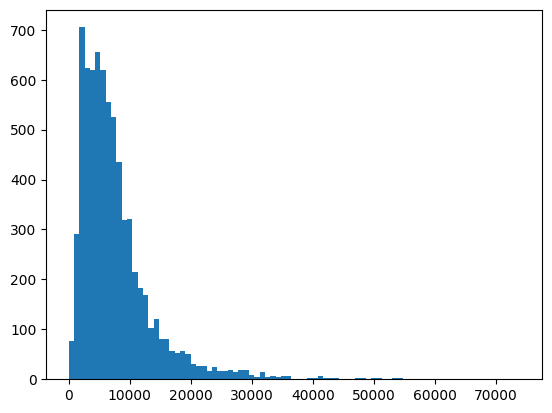
\includegraphics[width=.48\textwidth]{Images/govreport-wordcount.jpg}
	\caption{GovReport word counts}
	\label{fig:govreport}
\end{figure}


\subsection*{BigPatent}

Not used yet. \nocite{sharma-etal-2019-bigpatent}

\section{Methods used}


\subsection{Central truncation}

\begin{frame}{Central Truncation}

	\begin{itemize}
		\item The most common and straightforward approach used in practice to handle
		texts exceeding the context size.
		\item Generally, sequences are truncated from the end before processing.
		\item Some studies show that truncating the middle produced better results
		\citep{sun2019fine, worsham-kalita-2018-genre}.
		\item We keep a fraction of the tokens from the head and the tail, i.e. truncate
		the middle.
		\item Hyperparameter $head\_size \in [0, 1]$ controls the fraction of tokens taken
		from the head.
	\end{itemize}

\end{frame}


\subsection{Document Skimming}

\begin{frame}{Document Skimming}

	\begin{itemize}
		\item This approach is inspired by the fast reading technique "skimming".
		\item It involves reading while skipping some parts of the text for efficiency.
		\item Reader attempts to skip the redundant or irrelevant parts.
	\end{itemize}

	\vskip .5cm
	\begin{figure}
		\centering
		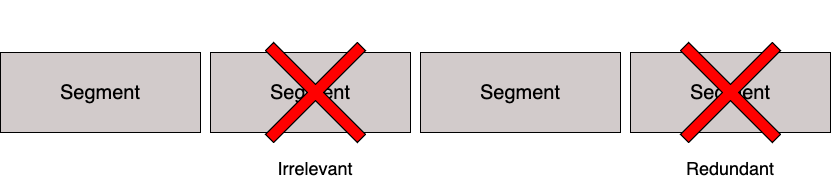
\includegraphics[width=\textwidth]{Images/skim.png}
	\end{figure}

\end{frame}

\begin{frame}{Document Skimming (contd.)}

	\begin{itemize}
		\item This method involves uniformly sampling the text segments to fill the LLM's
		context size.
		\item This ensures we capture details from every part of the text.
		\item A similar approach is taken by \citet{wang2024videoagent} to develop
		VideoAgent for QA on long videos.
	\end{itemize}

	\vskip 1cm

	\begin{figure}
		\centering
		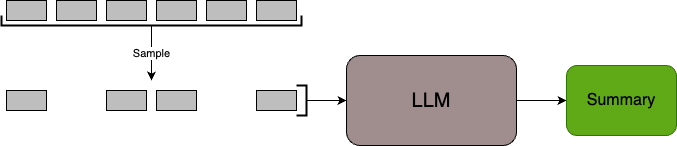
\includegraphics[width=1\textwidth]{Images/doc-skim.png}
	\end{figure}

\end{frame}


\subsection{Summarization w/ Extraction}

\begin{frame}{Summarization with Keyword Extraction}

	\begin{itemize}
		\item Instead of randomly sampling the text segments, we can make use of important
		keywords or phrases from the text for sampling.
		\item This can be achieved by using extractive summarization algorithms that can
		efficiently handle very long texts.
		\item We can then compute a probability distribution for the segments using
		similarity scores.
		\item We will be experimenting with: TextRank, LexRank, PacSum, Luhn's algorithm,
		and SummaRuNNer.
	\end{itemize}

\end{frame}


% \subsection{Pipeline 2}

% \begin{frame}{Pipeline 2}
	
% 	\begin{itemize}
% 		\item This pipeline is based on \textbf{Document Skimming}, i.e. skipping over some parts
% 		of the document.
% 		\item<2-> We start by segmenting the text into chunks of sentences.
% 		\item<3-> The size of a segment is decided by number of words in it.
% 		\item<4-> Each segment must have at least $min\_words$ words, which is a
% 		hyperparameter.
% 	\end{itemize}

% \end{frame}

% \begin{frame}{Pipeline 2 (contd.)}
	
% 	\begin{itemize}
% 		\item We then uniformly sample the segmented text to fill the context size.
% 		\item<2-> Each segment has a probability $p$ of being selected.
% 		\item<3-> $ p = context\_size / total\_tokens $
% 		(derivation provided in report)
% 		\item<4-> The selected segments are then concatenated with segment delimiters
% 		and sent to the summarizer.
% 	\end{itemize}

% \end{frame}


% \subsection{Pipeline 3}

% \begin{frame}{Pipeline 3}

% 	\begin{itemize}
% 		\item This pipeline is also based on \textbf{Document Skimming} and is a modification
% 		of \textbf{Pipeline 2}.
% 		\item<2-> After sampling the segments, segments similar to previously picked
% 		segments are removed.
% 		\item<3-> This is done by comparing the segment embeddings generated by
% 		a sentence transformer from Hugging Face.
% 		\item<4-> We linearly traverse the sampled segments and track the mean of the
% 		sentence embeddings.
% 		\item<5> Hyperparameter $threshold \in (0, 1]$: Segment $i$ is removed if
% 		\[ \mathrm{cos\_sim}(mean\_emb, emb_i) \ge threshold \]
% 	\end{itemize}

% \end{frame}


% \subsection{Pipeline 4}

% \begin{frame}{Pipeline 4}

% 	\begin{itemize}
% 		\item This pipeline is also a modification of \textbf{Pipeline 2} and is similar to
% 		\textbf{Pipeline 3}.
% 		\item<2-> Instead of removing similar segments after sampling, we first remove similar
% 		segments and then uniformly sample the segments.
% 		\item<3-> Although this pipeline might be slower than \textbf{Pipeline 3}, it ensures
% 		better utilization of the LLM's context size.
% 	\end{itemize}
	
% \end{frame}

\section{Experimental Findings}
	\label{sec:findings}


	\begin{table*}[!ht]
		\centering

		\begin{tabular}{c c c c c}
			\hline
			Model & ROUGE-1 & ROUGE-2 & ROUGE-L & BERTScore \\
			\hline
			BART w/ Unlimiformer (1,024) & 53.4 & 22.5 & 22.5 & 66.0 \\
			PRIMERA w/ Unlimiformer (4,096) & 56.5 & 24.8 & 26.3 & 67.7 \\
			Hepos (10,240) & 51.34 & 19.09 & \textbf{48.73} & - \\
			PEGASUS-X w/ Staggered & 60.3 & \textbf{30.0} & 31.5 & - \\
			Block-Local Attention (16k) & & & & \\
			LLaMA-7B w/ Positional & 60.0 & 28.0 & 29.5 & - \\
			Interpolation (15k) & & & & \\
			\hline
			Summarization w/ Extraction & \textbf{61.99} & 18.52 & 38.46 & \textbf{86.20} \\
			+ GPT-3.5 Turbo (4,096) & & & & \\
			Central truncation + LongT5 (4,096) & 46.20 & 4.38 & 38.27 & \textbf{82.19} \\
			Skimming w/ post-sampling & 46.76 & 4.56 & 39.61 & \textbf{81.96} \\
			removal + LongT5 (4,096) & & & & \\
			\hline
		\end{tabular}

		\caption{Automatic evaluation results on the GovReport dataset. Context size of the models are
		mentioned in parentheses. The best score in each metric category is highlighted in \textbf{bold}.}
		\label{tab:govreport}
	\end{table*}

	\begin{table*}[!ht]
		\centering

		\begin{tabular}{c c c c c}
			\hline
			Model & ROUGE-1 & ROUGE-2 & ROUGE-L & BERTScore \\
			\hline
			BigBird-Pegasus (16k) & \textbf{60.64} & \textbf{42.46} & \textbf{50.01} & - \\
			\hline
			Skimming w/ pre-sampling & 27.40 & 3.31 & 21.25 & \textbf{82.62} \\
			removal + GPT-3.5 Turbo (4,096) & & & & \\
			Central truncation + GPT-3.5 Turbo (4,096) & 27.77 & 3.09 & 20.56 & \textbf{82.57} \\
			Skimming w/ post-sampling & 26.16 & 2.13 & 20.21 & \textbf{82.40} \\
			removal + GPT-3.5 Turbo (4,096) & & & & \\
			\hline
		\end{tabular}

		\caption{Automatic evaluation results on the BigPatent dataset. Context size of the models are
		mentioned in parentheses. The best score in each metric category is highlighted in \textbf{bold}.}
		\label{tab:bigpatent}
	\end{table*}

	We test our pipelines with the following models: \textbf{BART} (Bidirectional
	and Autoregressive Transformer) \cite{lewis-etal-2020-bart} fine-tuned on the
	CNN/Daily Mail dataset \cite{nallapati2016abstractive} with a context size of 1024,
	\textbf{LongT5} \cite{guo2021longt5}, a variant of T5 (Text-to-Text Transfer
	Transformer) \cite{raffel2020exploring}, fine-tuned on the BookSum dataset with
	a context size of 4096, and \textbf{GPT-3.5 Turbo} \cite{brown2020language} with a
	context size of 4096.

	We compare our results with the state-of-the-art summarization models on the GovReport dataset,
	including Unlimiformer \cite{bertsch2023unlimiformer} integrated with BART
	\cite{lewis-etal-2020-bart} and PRIMERA \cite{beltagy2020longformer}, Hepos
	\cite{huang-etal-2021-efficient}, PEGASUS-X with staggered block-local attention
	\cite{phang2022investigating}, extended	LLaMA-7B with positional interpolation
	\cite{chen2023extending}.
	We also compare our results with BigBird-Pegasus \cite{zaheer2020big} on the BigPatent dataset.
	Refer to \autoref{tab:govreport} and \autoref{tab:bigpatent} for results on the GovReport and 
	BigPatent datasets, respectively.

	We were unable to confirm the BERTScores of our baselines, except for Unlimiformer, due to
	unavailability of code or computational limitations.


	\subsection*{Time complexity analysis}

		We evaluate the time complexity of our methods by measuring the mean time taken to process a
		document (excluding the time taken by the model to generate the summaries).
		We find that Central Truncation (\ref{method:truncation}) and Document Skimming
		(\ref{method:skimming}) take approximately the same time.
		Skimming with post-sampling removal takes slightly more time than the other two methods.
		We can see a significant increase in time taken by Skimming with pre-sampling removal
		and Summarization with Keyword Extraction (\ref{method:keyword}) due to the additional
		computations required.
		\autoref{fig:times} illustrates the average time taken by our methods.
		Check \autoref{tab:encoder-times} for exact values rounded off to two decimal places.

		\begin{figure}[!ht]
			\centering
			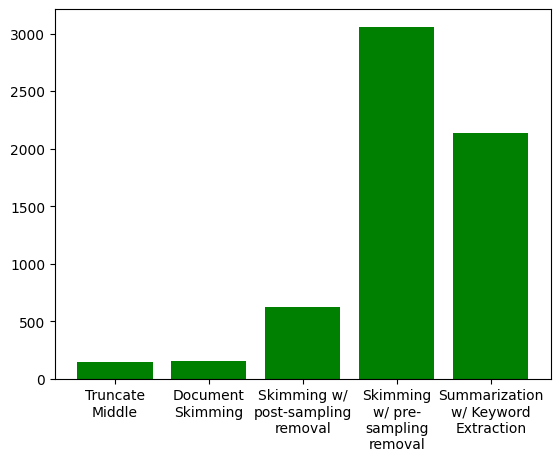
\includegraphics[width=.48\textwidth]{Images/encoder-times.png}
			\caption{Mean time taken per document using BART tokenizer on BigPatent dataset}
			\label{fig:times}
		\end{figure}

		\begin{table}[!ht]
			\centering

			\begin{tabular}{c c}
				\hline
				Method & Mean time taken \\
				\hline
				Central Truncation & 142.50 ms \\
				Document Skimming & 155.42 ms \\
				Skimming w/ post- & 625.17 ms \\
				sampling removal & \\
				Skimming w/ pre- & 3059.63 ms \\
				sampling removal & \\
				Summarization & 2131.40 ms \\
				w/ Extraction & \\
				\hline
			\end{tabular}

			\caption{Mean time taken per document using BART tokenizer on BigPatent dataset}
			\label{tab:encoder-times}
		\end{table}

\section{Future Work}

	\begin{frame}{Future Work}

		\begin{itemize}
			\item Future work can be focused on using better text segmentation techniques.
			\item We use nltk.sent\_tokenize with a threshold on the minimum number of words
			in a segment.
			\item We also encourage experimenting with different ways to utilize keywords from
			the document.
		\end{itemize}

	\end{frame}

\begin{frame}{References}
\tiny

% \nocite{*}
\bibliography{../Report/anthology}
\bibliographystyle{../Report/acl_natbib}
  
\end{frame}

\section{Questions}

\begin{frame}
  \centering

  \huge Thank you for listening!
  \vskip .5cm
  \large Feel free to ask questions

\end{frame}


\end{document}
